% ideias:
% etimologia prosodia
% rant bret victor
% objetivo: pegar o que há de mais moderno na fonologia pro português e colocar
% num sistema tts!

\documentclass{beamer}

\usepackage[utf8]{inputenc}     % Encoding certo
\usepackage[brazilian]{babel}   % Hifenização e dicionário

\usepackage{algorithm}
\usepackage{algorithmic}
\usepackage{amsmath}
\usepackage{amsfonts}
\usepackage{amssymb}
\usepackage{tikz}
\usepackage{tipa}
\usetikzlibrary{positioning, fit, arrows.meta, backgrounds}

\def\signed #1{{\leavevmode\unskip\nobreak\hfil\penalty50\hskip2em
  \hbox{}\nobreak\hfil(#1)%
  \parfillskip=0pt \finalhyphendemerits=0 \endgraf}}

\newsavebox\mybox
\newenvironment{aquote}[1]
  {\savebox\mybox{#1}\begin{quote}}
  {\signed{\usebox\mybox}\end{quote}}

\setbeamertemplate{navigation symbols}{}  % Esconde o menu tosco
\usetheme{Madrid}
\useinnertheme{rectangles}
\usefonttheme{professionalfonts}
% \usefonttheme{serif}            % A versão sem serifa é horrível
\usepackage{times}

\setbeamertemplate{blocks}[default]

\title[Geração de prosódia]{Geração de prosódia para o português brasileiro em sistemas text-to-speech}

\author{Felipe Cortez de Sá}
\date{Junho de 2018}
\institute[UFRN]{Universidade Federal do Rio Grande do Norte}

\begin{document}

\begin{frame}
  \titlepage
\end{frame}

\begin{frame}{Resumo}
  \tableofcontents
\end{frame}

\section{Introdução}
\begin{frame}
  \begin{aquote}{Leonhard Euler, 1761}
    It would be a considerable invention indeed, that of
    a machine able to mimic speech, with its sounds and articulations.
    I think it is not impossible."
  \end{aquote}
\end{frame}

\begin{frame}{Motivação}
  \begin{itemize}
    \item Euler e Wolfgang von Kempelen
    \item \emph{Voice User Interfaces}
        \begin{itemize}
            \item \emph{Apple - Siri}
            \item \emph{Google Assistant}
            \item \emph{Microsoft - Cortana}
            \item \emph{Amazon - Alexa}
        \end{itemize}
    \item Acessibilidade
    \item Ensino de linguagens
    \item Estudo de linguística
    \item Prosódia afetiva
  \end{itemize}
\end{frame}

\section{Fundamentação teórica}
\subsection{Prosódia}
\begin{frame}{Prosódia}
  \begin{itemize}
    \item pros (verso) - odé (canto)
     \item Suprassegmental
     \item Frequência
     \item Duração
     \item Intensidade
  \end{itemize}
\end{frame}

\begin{frame}{Prosódia}
    \begin{figure}
      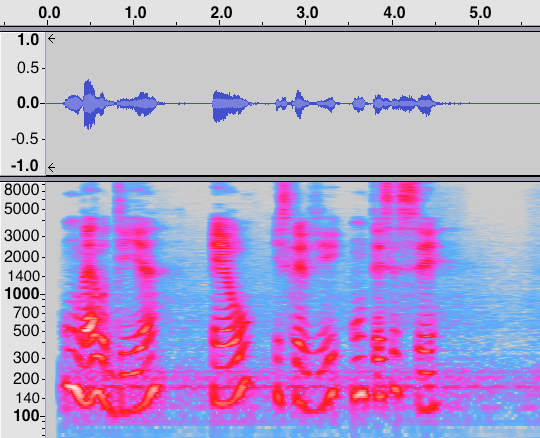
\includegraphics[scale=0.50]{espectro.png}
    \end{figure}
\end{frame}

\begin{frame}{Função prosódica}
  \begin{itemize}
    % \citeonline{taylor2009} argumenta que uma das dificuldades do desenvolvimento de um bom modelo de prosódia se deve à falta de consideração da função comunicativa da fala, isto é, comumente análises são feitas ignorando o contexto da intenção do locutor. Apresenta, então, as três principais funções comunicativas para prosódia, descritas a seguir.
    \item Suprassegmental
    \item Afetiva
    \item Aumentativa
  \end{itemize}
\end{frame}

\subsection{Sistemas text-to-speech}
\begin{frame}{Sistemas text-to-speech}
  \begin{figure}[!htbp]
  \centering
  \scalebox{0.80}{
      \begin{tikzpicture}[auto, >={Latex[inset=0pt, length=3mm, angle'=28,round]}, box/.style={draw,rounded corners,text width=4.5cm,align=center}]
      \node[] (txt) {Texto};
      \node[box, right=of txt] (nlp)
          {Processamento de linguagem natural};
      \node[box, right=of nlp] (dsp)
          {Processamento digital de sinais};
      \node[right=of dsp] (fal)
          {Fala};

          \node[box, fit=(nlp)(dsp), label=Sistema \emph{text-to-speech}] (tts) {};

      \draw[->] (txt) -- (nlp);
      \draw[->] (nlp) -- (dsp);
      \draw[->] (dsp) -- (fal);
      \end{tikzpicture}
  }
  \label{fig:tts-arch}
  \end{figure}

\end{frame}

\begin{frame}{Arquitetura}
  \begin{itemize}
    \item Front end
    \begin{itemize}
      \item Normalização de texto
      \item Conversão grafema-fone
      \item Geração de prosódia
    \end{itemize}
    \item Back end
    \begin{itemize}
      \item Síntese articulatória
      \item Síntese por formantes
      \item Síntese concatenativa
      \item Síntese por Hidden Markov Models e Deep Neural Networks
    \end{itemize}
  \end{itemize}
\end{frame}

\begin{frame}{Front end}
  \begin{itemize}
    \item Normalização de texto
      \begin{itemize}
        \item A conta deu R\$ 20, V. Exa. Pode conferir?
      \end{itemize}
    \item Conversão grafema-fone
      \begin{itemize}
        \item Gosto de pão
        \item \textipa{[gOstu]} (gósto)
        \item \textipa{[gostu]} (gôsto)
      \end{itemize}
    \item Geração de prosódia
  \end{itemize}
\end{frame}

\begin{frame}{O desafio da geração de prosódia}
  \pause
    \begin{figure}
      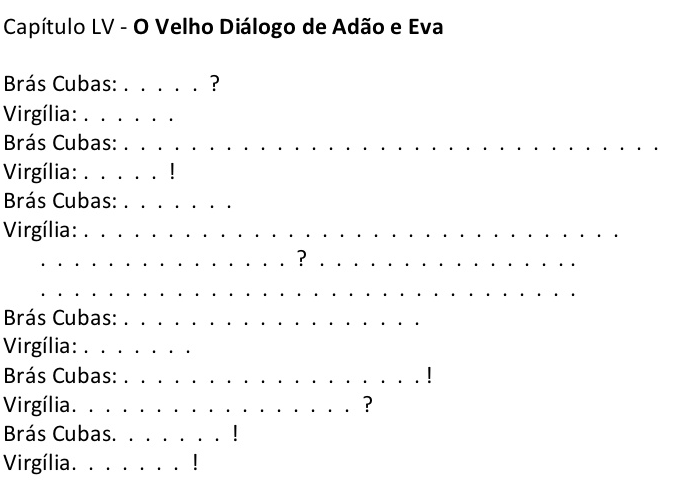
\includegraphics[scale=0.40]{machado.png}
    \end{figure}
\end{frame}

\begin{frame}{Geração de prosódia}
      \begin{itemize}
        \item Heurísticas derivadas a mão
        \item Sistemas baseados em análise gramatical
        \item Métodos baseados em corpus
      \end{itemize}
\end{frame}

\begin{frame}{Back end}
\begin{itemize}
  \item Síntese articulatória
  \item Síntese por formantes
  \item Síntese concatenativa
  \item Síntese por Hidden Markov Models e Deep Neural Networks
\end{itemize}
\end{frame}

% • And since it is almost mathematically proven that speech = voice passing
% through openings it follows that for a speaking machine you need nothing else
% but
%    • a lung
%    • a glottis
%    • a mouth

\begin{frame}{Máquina de Wolfgang von Kempelen (1778)}
    \begin{figure}
      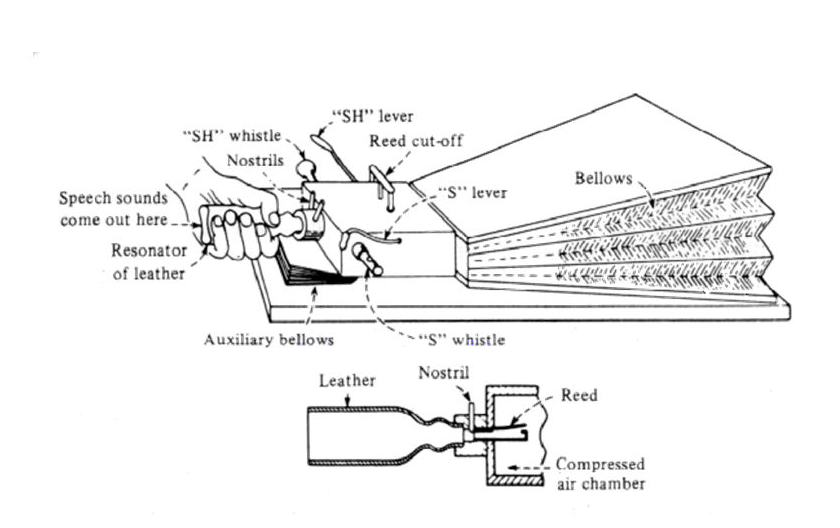
\includegraphics[scale=0.40]{kempelen.png}
    \end{figure}
\end{frame}

\begin{frame}{Articulatória}
    \begin{figure}
      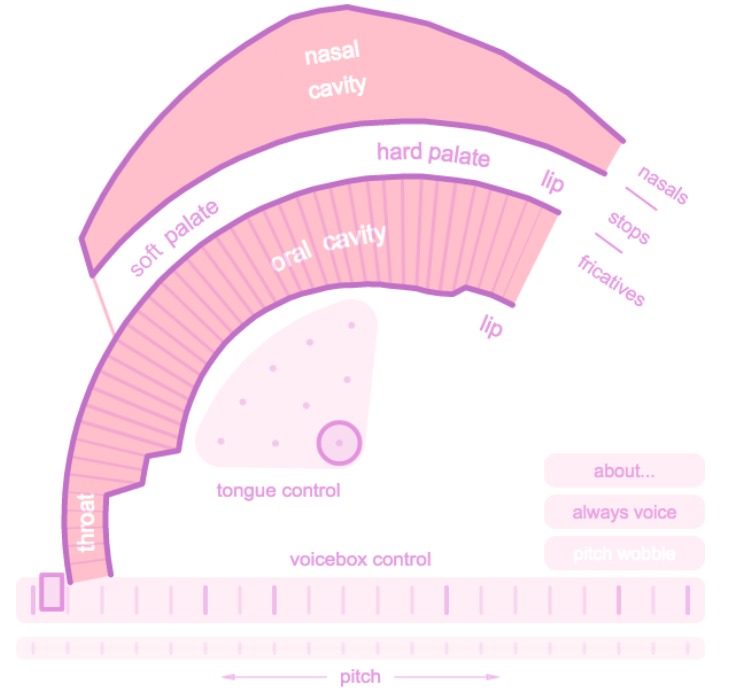
\includegraphics[scale=0.30]{pinktrombone.png}
    \end{figure}
\end{frame}

\begin{frame}{Formantes}
    \begin{figure}
      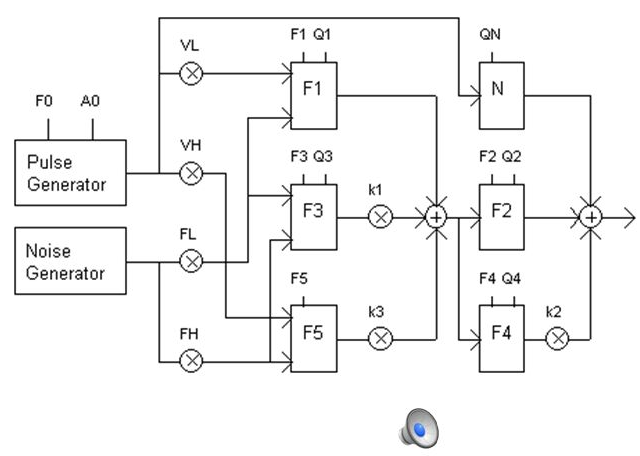
\includegraphics[scale=0.40]{klatt.png}
    \end{figure}
\end{frame}

\begin{frame}{Concatenativa}
    \begin{figure}
      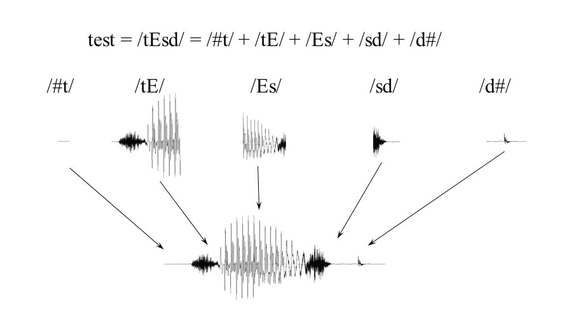
\includegraphics[scale=0.60]{concatenative.png}
    \end{figure}
\end{frame}

\begin{frame}{HMM}
    \begin{figure}
      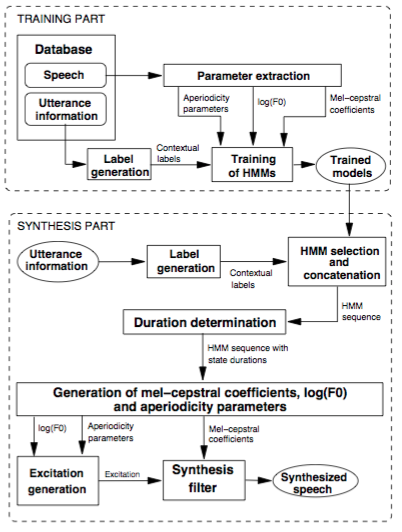
\includegraphics[scale=0.38]{hmm.png}
    \end{figure}
\end{frame}

\begin{frame}{Sistemas TTS para o português brasileiro}
  \begin{itemize}
      \item Aiuruetê (1997) -- curvas de frequência pré-definidas
      \item eSpeakNG (2006) -- \emph{pre-head, head, nucleus, tail}
      \item Couto et al (2010) -- probabilístico
      \item LianeTTS (2011) -- partes do discurso
  \end{itemize}
\end{frame}

\begin{frame}{Analisando prosódia}
  \begin{itemize}
  \item ToBI -- Tone Breaks and Indices
  \item DaTo -- Dynamic Tones
  \item INTSINT -- International Transcription System for Intonation
  \end{itemize}
\end{frame}

\begin{frame}{ToBI}
    \begin{figure}
      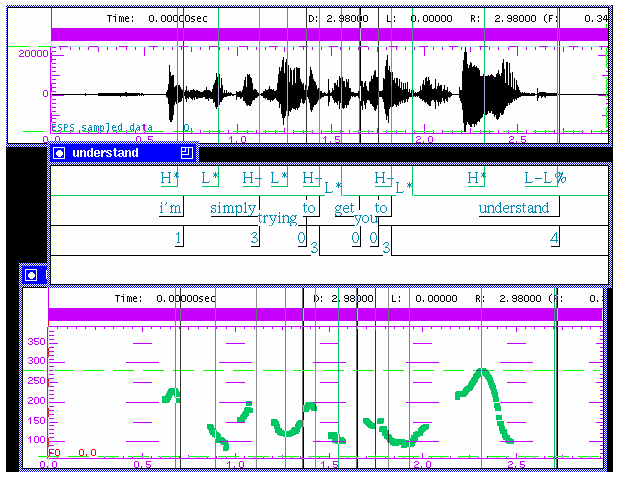
\includegraphics[scale=0.40]{tobi.png}
    \end{figure}
\end{frame}

\begin{frame}{DaTo}
    \begin{figure}
      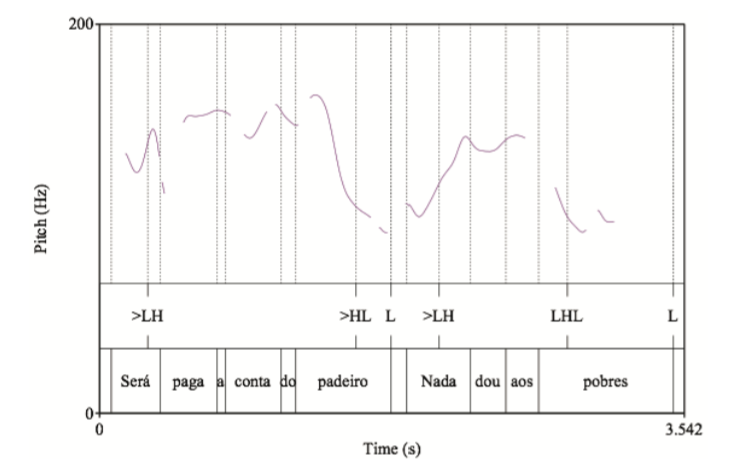
\includegraphics[scale=0.40]{dato.png}
    \end{figure}
\end{frame}

\begin{frame}{INTSINT}
    \begin{figure}
      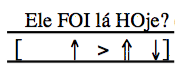
\includegraphics[scale=0.80]{intsint.png}
    \end{figure}
\end{frame}

\begin{frame}{Complementando texto}
  \begin{itemize}
  \item SSML -- Speech Synthesis Markup Language
  \item EmotionML
  \item Anotações entoacionais
  \end{itemize}
\end{frame}

\begin{frame}{SSML}
    \begin{figure}
      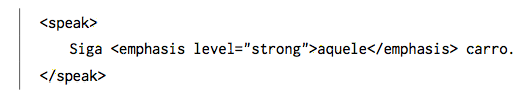
\includegraphics[scale=0.60]{ssml.png}
    \end{figure}
\end{frame}

\begin{frame}{EmotionML}
    \begin{figure}
      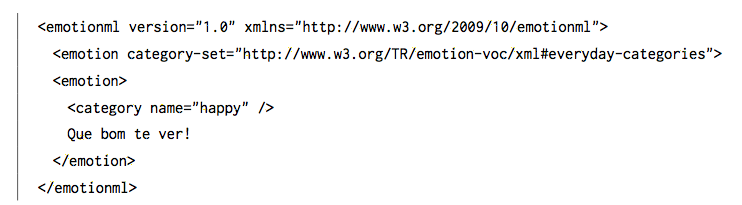
\includegraphics[scale=0.40]{emotionml.png}
    \end{figure}
\end{frame}

\begin{frame}{Anotações manuais}
    \begin{figure}
      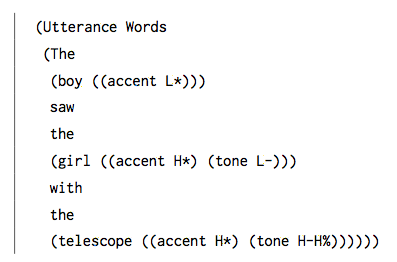
\includegraphics[scale=0.60]{manual.png}
    \end{figure}
\end{frame}

\section{Implementação}

\begin{frame}{Arquitetura}
\begin{figure}[!htbp]
\centering
\scalebox{0.80}{
    \begin{tikzpicture}[auto, >={Latex[inset=0pt, length=3mm, angle'=28,round]}, box/.style={draw,rounded corners,text width=3.0cm,align=center}]
    \node[] (txt) {Texto};
    \node[box, right=of txt] (esp)
        {eSpeakNG};
    \node[box, right=of esp, line width=1.6pt] (con)
        {Conversão eSpeakNG para MBROLA};
    \node[box, right=of con, line width=1.6pt] (sin)
        {INTSINT};
    \node[above=of con] (ano)
        {Texto anotado};

    \node[box, below=of sin, line width=1.6pt] (ser)
        {Servidor};

    \node[box, left=of ser] (mbr)
        {MBROLA};

    \node[box, below=of ser, line width=1.6pt] (int)
        {Interface gráfica};

    \draw[->] (ano) -| (txt);
    \draw[->] (ano) -- (con);
    \draw[->] (txt) -- (esp);
    \draw[->] (esp) -- (con);
    \draw[->] (con) -- (sin);

    \draw[->] (sin) -- (ser);
    \draw[->] (mbr) -- (ser);

    \draw[<->] (ser) -- (int);

    \end{tikzpicture}
}
\label{fig:arch}
\end{figure}
\end{frame}

\begin{frame}{eSpeakNG}
  \begin{figure}
    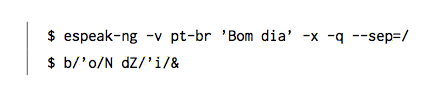
\includegraphics[scale=0.60]{espeak.png}
  \end{figure}
\end{frame}

\begin{frame}{Conversão de fones}
  \begin{figure}
    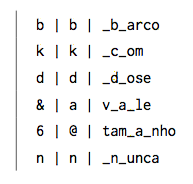
\includegraphics[scale=0.60]{conversao.png}
  \end{figure}
\end{frame}

\begin{frame}
\begin{table}[htb]
	\center
	{
		\begin{tabular}{l|l}
			\hline
			Regra       & Cálculo \\
			\hline
            Top         & $ \text{key} \times \sqrt{2^{range}} $ \\
            Middle      & $ \text{key} $ \\
            Bottom      & $ \text{key} / \sqrt{2^{range}} $ \\
			\hline
            Higher      & $ \sqrt{P_{i - 1} \times T} $ \\
            Same        & $ P_{i - 1} $ \\
            Lower       & $ \sqrt{P_{i - 1} \times B} $ \\
			\hline
            Upstepped   & $ \sqrt{P_{i - 1} \times  \sqrt{P_{i - 1} \times  T}} $ \\
            Downstepped & $ \sqrt{P_{i - 1} \times  \sqrt{P_{i - 1} \times  B}} $ \\
			\hline
		\end{tabular}
	}
	\label{tab:intsint}
\end{table}
\end{frame}

\begin{frame}{MBROLA}
  \begin{figure}
    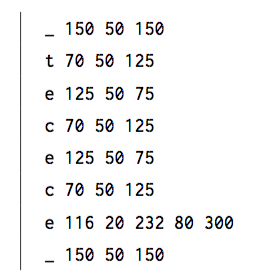
\includegraphics[scale=0.60]{mbrola.png}
  \end{figure}
\end{frame}

\begin{frame}{Concatenando dífonos}
    \begin{figure}
      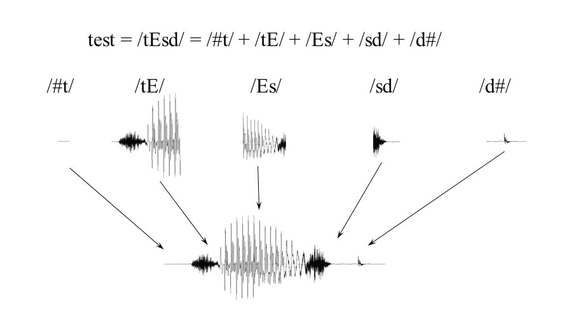
\includegraphics[scale=0.60]{concatenative.png}
    \end{figure}
\end{frame}

\begin{frame}
\begin{table}[htb]
  Demonstração!
\end{table}
\end{frame}

\begin{frame}{Trabalhos futuros}
  \begin{itemize}
    \item Adicionar suporte a outros modelos de análise entoacional
    \item Usar \emph{Natural Language Understanding} para estimar prosódia
    \item Gerar prosódia a partir de marcação SSML
    \item Criação de corpus anotado com prosódia para o português brasileiro
  \end{itemize}
\end{frame}

\section{Perguntas}
\begin{frame}{Perguntas}
\begin{aquote}{Miles Davis}
If you understood everything I said, you'd be me
\end{aquote}
\end{frame}

\end{document}
